% 2006_jiangxi_liberal_q20_fig1: trirectangular tetrahedron O-ABC, E midpoint of OC
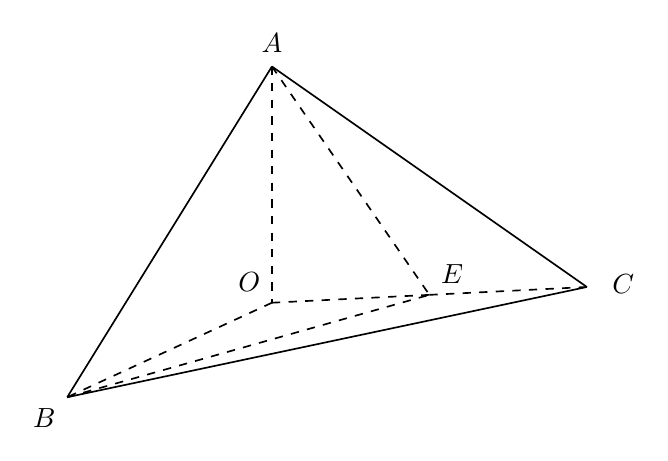
\begin{tikzpicture}[x=1cm,y=1cm,font=\normalsize,
  geometry edge/.style={solid,line width=.6pt},
  geometry label/.style={font=\normalsize,inner sep=2pt}]
\coordinate (O) at (0,0);
\coordinate (A) at (0.0000000000,3.0000000000);
\coordinate (B) at (-2.6,-1.2);
\coordinate (C) at (4.0,0.2);
\coordinate (E) at (2.0,0.1);
% hidden edges (dashed)
\draw[geometry edge,dashed] (A)--(O);
\draw[geometry edge,dashed] (O)--(B);
\draw[geometry edge,dashed] (O)--(E);
\draw[geometry edge,dashed] (E)--(C);
\draw[geometry edge,dashed] (A)--(E);
\draw[geometry edge,dashed] (B)--(E);
% visible faces (solid)
\draw[geometry edge] (A)--(B);
\draw[geometry edge] (A)--(C);
\draw[geometry edge] (B)--(C);
% labels offset from strokes
\node[geometry label,above] at (A) [yshift=3pt] {$A$};
\node[geometry label,above left=2pt] at (O) {$O$};
\node[geometry label,below left] at (B) [xshift=-2pt,yshift=-2pt] {$B$};
\node[geometry label,right] at (C) [xshift=7pt,yshift=1pt] {$C$};
\node[geometry label,above right] at (E) [xshift=2pt,yshift=2pt] {$E$};
\end{tikzpicture}
